\documentclass[conference]{IEEEtran}
\usepackage[utf8]{inputenc}
\usepackage[T1]{fontenc}
\usepackage{amsmath,amssymb}
\usepackage{graphicx}
\usepackage{booktabs}
\usepackage{multirow}
\usepackage[hidelinks]{hyperref}
\graphicspath{{figures/}}

\newcommand{\Fmax}{\bar{F}}
\setlength{\textfloatsep}{9pt plus 2pt minus 4pt}
\setlength{\dbltextfloatsep}{9pt plus 2pt minus 4pt}
% generated by experiments/make_numbers.py -- do not edit
\newcommand{\agilityFastRate}{3/6}
\newcommand{\agilityFastV}{0.25}
\newcommand{\agilityRate}{10/10}
\newcommand{\agilityV}{0.23}
\newcommand{\allMotorMass}{48.6}
\newcommand{\authGaitAll}{0.00}
\newcommand{\authGaitBom}{0.00}
\newcommand{\authGaitHip}{0.87}
\newcommand{\authGaitKnee}{0.61}
\newcommand{\authHomeAll}{1.01}
\newcommand{\authHomeBom}{0.66}
\newcommand{\authShortGaitAll}{10}
\newcommand{\authShortGaitBom}{13}
\newcommand{\authShortHomeAll}{0}
\newcommand{\authShortHomeBom}{6}
\newcommand{\bearingMass}{1.89}
\newcommand{\bearingPerDof}{70}
\newcommand{\benchAnkleArmA}{55}
\newcommand{\benchAnkleArmB}{66}
\newcommand{\benchAnkleMoment}{16}
\newcommand{\benchLegSink}{12}
\newcommand{\benchLegT}{41}
\newcommand{\benchLegTTwo}{55}
\newcommand{\benchWaistSink}{24}
\newcommand{\bomMass}{16.1}
\newcommand{\bomMassFixed}{19.4}
\newcommand{\carryHinEight}{6.0}
\newcommand{\carryHinSixteen}{8.0}
\newcommand{\carryHinSlope}{16}
\newcommand{\carryHinTwelve}{6.0}
\newcommand{\carryHybEight}{1.5}
\newcommand{\carryHybSixteen}{3.0}
\newcommand{\carryHybSlope}{53}
\newcommand{\carryHybTwelve}{2.0}
\newcommand{\cellChainDroop}{29}
\newcommand{\cellChainMax}{5}
\newcommand{\cellChainPer}{5.9}
\newcommand{\cgCables}{306}
\newcommand{\cgCellStruts}{39}
\newcommand{\cgClusterStruts}{27}
\newcommand{\cgDof}{210}
\newcommand{\cgLoadFail}{5}
\newcommand{\cgNodeLoad}{637}
\newcommand{\cgNodeMargin}{3.7}
\newcommand{\cgPreNeeded}{1000}
\newcommand{\cgPreSettle}{48}
\newcommand{\cgSettle}{6}
\newcommand{\cgStruts}{66}
\newcommand{\cpayAllCiHi}{83}
\newcommand{\cpayAllCiLo}{65}
\newcommand{\cpayAllPct}{75}
\newcommand{\cpayAllRate}{60/80}
\newcommand{\cpayEightCiHi}{89}
\newcommand{\cpayEightCiLo}{40}
\newcommand{\cpayEightRate}{7/10}
\newcommand{\cpayEightV}{0.19}
\newcommand{\cpayFourCiHi}{83}
\newcommand{\cpayFourCiLo}{31}
\newcommand{\cpayFourRate}{6/10}
\newcommand{\cpayFourV}{0.19}
\newcommand{\cpaySixCiHi}{89}
\newcommand{\cpaySixCiLo}{40}
\newcommand{\cpaySixRate}{7/10}
\newcommand{\cpaySixV}{0.20}
\newcommand{\cpaySixteenCiHi}{98}
\newcommand{\cpaySixteenCiLo}{60}
\newcommand{\cpaySixteenRate}{9/10}
\newcommand{\cpaySixteenV}{0.17}
\newcommand{\cpayTenCiHi}{83}
\newcommand{\cpayTenCiLo}{31}
\newcommand{\cpayTenRate}{6/10}
\newcommand{\cpayTenV}{0.20}
\newcommand{\cpayTwelveCiHi}{89}
\newcommand{\cpayTwelveCiLo}{40}
\newcommand{\cpayTwelveRate}{7/10}
\newcommand{\cpayTwelveV}{0.19}
\newcommand{\cpayTwentyCiHi}{98}
\newcommand{\cpayTwentyCiLo}{60}
\newcommand{\cpayTwentyRate}{9/10}
\newcommand{\cpayTwentyV}{0.17}
\newcommand{\cpayTwoCiHi}{98}
\newcommand{\cpayTwoCiLo}{60}
\newcommand{\cpayTwoRate}{9/10}
\newcommand{\cpayTwoV}{0.20}
\newcommand{\distalN}{10}
\newcommand{\distalOk}{6}
\newcommand{\distalRate}{6/10}
\newcommand{\distalSpeed}{0.17}
\newcommand{\eOneBWRigidCrash}{14}
\newcommand{\eOneBWRigidStumble}{5}
\newcommand{\eOneBWTsgCrash}{36}
\newcommand{\eOneBWTsgStumble}{5}
\newcommand{\eOneCrossover}{0.2}
\newcommand{\eOneDeltaHeldCrash}{+3}
\newcommand{\eOneDeltaHeldStumble}{+2}
\newcommand{\eOneDeltaPassiveCrash}{+154}
\newcommand{\eOneDeltaPassiveStumble}{+14}
\newcommand{\eOneHeldRigidCrash}{4133}
\newcommand{\eOneHeldRigidStumble}{1820}
\newcommand{\eOneHeldTsgCrash}{4262}
\newcommand{\eOneHeldTsgStumble}{1853}
\newcommand{\eOneMismatched}{20}
\newcommand{\eOnePassiveFell}{7}
\newcommand{\eOnePassiveN}{7}
\newcommand{\eOnePassiveRigidCrash}{3785}
\newcommand{\eOnePassiveRigidStumble}{1273}
\newcommand{\eOnePassiveTsgCrash}{9629}
\newcommand{\eOnePassiveTsgStumble}{1454}
\newcommand{\eSixSummary}{Capping every joint at the torque the full cable network can deliver over the gait leaves the planner 7/10 successful walks at 0.17\,m/s; capping at the worst-case bound gives 3/6; and capping at what the 36-motor bill of materials can deliver gives 0/10. A gait therefore exists inside the envelope of the full network but not inside the envelope of the actuation set we specified: the shortfall is in the bill of materials, not in the topology.}
\newcommand{\eSixtendonallRate}{7/10}
\newcommand{\eSixtendonbomRate}{0/10}
\newcommand{\eSixtendonminRate}{3/6}
\newcommand{\eThreeAdvEight}{0/4}
\newcommand{\eThreeAdvFour}{4/4}
\newcommand{\eThreeAdvTwo}{4/4}
\newcommand{\eThreeBaseMargin}{1.01}
\newcommand{\eThreeBelowOne}{44}
\newcommand{\eThreeLegEight}{8/8}
\newcommand{\eThreeLegFour}{8/8}
\newcommand{\eThreeLegTwo}{8/8}
\newcommand{\eThreeRandEight}{8/8}
\newcommand{\eThreeRandFour}{8/8}
\newcommand{\eThreeRandTwo}{8/8}
\newcommand{\eThreeSinglesN}{15}
\newcommand{\eThreeSinglesOk}{15}
\newcommand{\extraMotorMass}{3.2}
\newcommand{\freeZend}{-0.03}
\newcommand{\freeZstart}{0.94}
\newcommand{\gaitClr}{42}
\newcommand{\hingeConstrainedDof}{57}
\newcommand{\hingeDof}{27}
\newcommand{\hingeDofCount}{27}
\newcommand{\hingeSegments}{14}
\newcommand{\hsCarryMax}{2.0}
\newcommand{\hsCarryUtil}{65}
\newcommand{\hsCarryWaistT}{88}
\newcommand{\hsPayEightRate}{3/10}
\newcommand{\hsPayEightV}{0.20}
\newcommand{\hsPayFiveRate}{9/10}
\newcommand{\hsPayFiveV}{0.18}
\newcommand{\hsPayTwelveRate}{0/10}
\newcommand{\hsPayTwelveV}{0.00}
\newcommand{\hsPayTwoRate}{10/10}
\newcommand{\hsPayTwoV}{0.18}
\newcommand{\hsSpdFortyFiveRate}{6/6}
\newcommand{\hsSpdFortyFiveV}{0.19}
\newcommand{\hsSpdSixtyRate}{0/6}
\newcommand{\hsSpdSixtyV}{0.00}
\newcommand{\hsSpdThirtyRate}{6/6}
\newcommand{\hsSpdThirtyV}{0.10}
\newcommand{\hybridAnkleDuty}{7}
\newcommand{\hybridAnklePeak}{250}
\newcommand{\hybridHipHw}{257}
\newcommand{\hybridJointDuty}{9}
\newcommand{\hybridJointHw}{0.8}
\newcommand{\hybridKneeHw}{142}
\newcommand{\hybridMass}{20.1}
\newcommand{\hybridRate}{10/10}
\newcommand{\hybridSpeed}{0.18}
\newcommand{\jcRAnkleRate}{5/5}
\newcommand{\jcRAnkleV}{0.21}
\newcommand{\jcRBothRate}{5/5}
\newcommand{\jcRBothV}{0.23}
\newcommand{\jcRWaistRate}{0/5}
\newcommand{\jcRWaistTunedRate}{4/5}
\newcommand{\jcRWaistTunedTorso}{1.28}
\newcommand{\jcRWaistTunedV}{0.18}
\newcommand{\jcRWaistV}{0.00}
\newcommand{\jointGeomElasticRope}{0.2}
\newcommand{\jointGeomElasticSoft}{67}
\newcommand{\jointImpactCableFive}{209}
\newcommand{\jointImpactCableTen}{282}
\newcommand{\jointImpactCableTwenty}{388}
\newcommand{\jointImpactDeltaFive}{27}
\newcommand{\jointImpactDeltaTen}{30}
\newcommand{\jointImpactDeltaTwenty}{32}
\newcommand{\jointImpactHi}{32}
\newcommand{\jointImpactLo}{27}
\newcommand{\jointImpactPinFive}{287}
\newcommand{\jointImpactPinTen}{404}
\newcommand{\jointImpactPinTwenty}{568}
\newcommand{\jointOverlapFrac}{0.2}
\newcommand{\jointOverlapMm}{60}
\newcommand{\jointPreRatioRope}{1.06}
\newcommand{\jointPreRatioSeries}{1.33}
\newcommand{\jointPreRatioSoft}{23.22}
\newcommand{\kModelMax}{2500}
\newcommand{\kModelMin}{600}
\newcommand{\kRopeMax}{7.1}
\newcommand{\kRopeMin}{0.3}
\newcommand{\kSeriesMax}{168}
\newcommand{\kSeriesMin}{20}
\newcommand{\lbCables}{135}
\newcommand{\lbDroop}{18}
\newcommand{\lbStruts}{18}
\newcommand{\membersMass}{5.64}
\newcommand{\nodeCount}{93}
\newcommand{\nodeMass}{0.84}
\newcommand{\numActuatable}{114}
\newcommand{\numCableEnds}{444}
\newcommand{\numDof}{27}
\newcommand{\numDrivenCables}{72}
\newcommand{\numEndpoints}{372}
\newcommand{\numMotors}{36}
\newcommand{\numMotorsFixed}{43}
\newcommand{\numPassiveCables}{42}
\newcommand{\numStruts}{60}
\newcommand{\numTendonCable}{222}
\newcommand{\numTendonTorque}{186}
\newcommand{\payTenRate}{10/10}
\newcommand{\payTenV}{0.19}
\newcommand{\physOneHeldFifty}{+73}
\newcommand{\physOneHeldFive}{-25}
\newcommand{\physOneHeldHundred}{+96}
\newcommand{\physOneHeldTen}{+1}
\newcommand{\physOneHeldThirty}{+53}
\newcommand{\physOneHeldTwenty}{+41}
\newcommand{\physOneLimpFifty}{+177}
\newcommand{\physOneLimpFive}{+112}
\newcommand{\physOneLimpHundred}{+197}
\newcommand{\physOneLimpTen}{+110}
\newcommand{\physOneLimpThirty}{+142}
\newcommand{\physOneLimpTwenty}{+113}
\newcommand{\physTwoCableRatio}{18}
\newcommand{\physTwoEngaged}{-2}
\newcommand{\physTwoHigh}{591}
\newcommand{\physTwoNoCables}{13}
\newcommand{\physTwoNominal}{615}
\newcommand{\physTwoZeroPre}{226}
\newcommand{\rHaveHip}{37.5}
\newcommand{\rHaveKnee}{47.6}
\newcommand{\rNeedHip}{53.3}
\newcommand{\realtimeFactor}{0.60}
\newcommand{\realtimeN}{142}
\newcommand{\ropeBLLeg}{12.8}
\newcommand{\ropeDMax}{4.0}
\newcommand{\ropeDMin}{1.0}
\newcommand{\ropeMass}{0.10}
\newcommand{\ropeUtilRms}{12}
\newcommand{\rpayEightRate}{5/6}
\newcommand{\rpayFourRate}{6/6}
\newcommand{\rpaySixRate}{5/6}
\newcommand{\rpaySixteenRate}{3/6}
\newcommand{\rpayTenRate}{3/6}
\newcommand{\rpayTwelveRate}{6/6}
\newcommand{\rpayTwentyRate}{4/6}
\newcommand{\rpayTwoRate}{3/6}
\newcommand{\shellAllowance}{0.26}
\newcommand{\singleLoopHip}{56}
\newcommand{\singleLoopKnee}{71}
\newcommand{\spdFortyFiveN}{10}
\newcommand{\spdFortyFiveOk}{1}
\newcommand{\spdFortyFiveRate}{1/10}
\newcommand{\spdFortyFiveV}{0.29}
\newcommand{\spdFortyN}{10}
\newcommand{\spdFortyOk}{3}
\newcommand{\spdFortyRate}{3/10}
\newcommand{\spdFortyV}{0.26}
\newcommand{\spdTenN}{10}
\newcommand{\spdTenOk}{0}
\newcommand{\spdTenRate}{0/10}
\newcommand{\spdTenV}{---}
\newcommand{\spdThirtyFiveN}{10}
\newcommand{\spdThirtyFiveOk}{6}
\newcommand{\spdThirtyFiveRate}{6/10}
\newcommand{\spdThirtyFiveV}{0.24}
\newcommand{\spdThirtyRate}{7/10}
\newcommand{\spdThirtyV}{0.21}
\newcommand{\spdTwentyN}{10}
\newcommand{\spdTwentyOk}{8}
\newcommand{\spdTwentyRate}{8/10}
\newcommand{\spdTwentyV}{0.13}
\newcommand{\stiffCablesRatio}{2.4}
\newcommand{\stiffCoHi}{115}
\newcommand{\stiffCoKnee}{96}
\newcommand{\stiffCoLo}{14}
\newcommand{\stiffCoRatio}{8.4}
\newcommand{\stiffGapRope}{1685}
\newcommand{\stiffGapSeries}{46}
\newcommand{\stiffLinearity}{0.5}
\newcommand{\stiffNoCables}{5.4}
\newcommand{\stiffNominal}{12.6}
\newcommand{\stiffPreHi}{16.6}
\newcommand{\stiffPreLo}{11.6}
\newcommand{\stiffPreRatio}{1.4}
\newcommand{\stiffProbe}{200}
\newcommand{\stiffSensTenHi}{+21}
\newcommand{\stiffSensTenLo}{+5}
\newcommand{\stiffZeroPre}{13.3}
\newcommand{\strutFittingMass}{0.36}
\newcommand{\strutLenMax}{589}
\newcommand{\strutLenMin}{32}
\newcommand{\strutLoadDrop}{3210}
\newcommand{\strutLoadStand}{90}
\newcommand{\strutLoadStumble}{485}
\newcommand{\strutMarginDrop}{0.7}
\newcommand{\strutMarginStand}{26.1}
\newcommand{\strutMarginStumble}{4.9}
\newcommand{\strutMassSized}{0.54}
\newcommand{\strutOdMax}{20}
\newcommand{\strutOdMin}{12}
\newcommand{\strutPeakN}{51}
\newcommand{\strutSpecMass}{1.03}
\newcommand{\strutTubeMass}{0.67}
\newcommand{\strutWall}{0.5}
\newcommand{\strutWeakestPcr}{2358}
\newcommand{\strutWorstMargin}{6.0}
\newcommand{\takeupMax}{202}
\newcommand{\takeupMin}{66}
\newcommand{\tendonSpecMass}{1.88}
\newcommand{\tensBusiestRms}{1020}
\newcommand{\tensNeedEight}{2557}
\newcommand{\tensNeedFour}{3310}
\newcommand{\tensNeedSixteen}{2782}
\newcommand{\tensNeedTwelve}{2559}
\newcommand{\tensNeedTwenty}{2619}
\newcommand{\tensNeeded}{2407}
\newcommand{\tensPeak}{1500}
\newcommand{\tensResid}{24}
\newcommand{\tensResidEight}{30}
\newcommand{\tensResidFour}{30}
\newcommand{\tensResidSixteen}{30}
\newcommand{\tensResidTwelve}{39}
\newcommand{\tensResidTwenty}{31}
\newcommand{\tensSatEight}{41}
\newcommand{\tensSatFour}{42}
\newcommand{\tensSatPct}{10.9}
\newcommand{\tensSatSixteen}{46}
\newcommand{\tensSatTwelve}{48}
\newcommand{\tensSatTwenty}{75}
\newcommand{\termMass}{1.78}
\newcommand{\walkCiHi}{89}
\newcommand{\walkCiLo}{40}
\newcommand{\walkCot}{3.3}
\newcommand{\walkN}{10}
\newcommand{\walkOk}{7}
\newcommand{\walkRate}{7/10}
\newcommand{\walkSpeed}{0.21}
\newcommand{\walkSpeedSd}{0.01}
\newcommand{\wcSix}{0}
\newcommand{\wcThree}{0}
\newcommand{\wcTotal}{14}


\title{MPC-Based Co-Design of a Hybrid Tensegrity Humanoid}

\author{\IEEEauthorblockN{Nikolaus Correll}
\IEEEauthorblockA{Department of Aerospace and Mechanical Engineering\\
University of Notre Dame\\
ncorrell@nd.edu}}

\begin{document}
\maketitle

\begin{abstract}
This paper examines how articulated joints and tensegrity structure should
be combined in a full-size humanoid robot. Three machines of identical
anthropometry are constructed in simulation and evaluated under a
receding-horizon iLQG controller: a pure tensegrity machine, a fully
hinged 27-DoF tendon-driven machine, and a hybrid of the two. A
wrench-closure analysis shows that a hinge-free cable joint requires both
overlapping cages and counter-wound cable families; without the latter
the cable set has no self-stress state and no balance controller can
exist. The pure tensegrity machine stands but presents 210 degrees of
freedom that no available planner stabilizes. The fully hinged machine
walks, but raises peak ground reaction at every drop height relative to a
rigid baseline, and its cable network does not meet its own torque
specification at gait poses. The hybrid places bearings at hips and knees and tensegrity joints at ankles and waist; at 1.68\,m and \hybridMass\,kg it walks at \hybridSpeed\,m/s in \hybridRate{} of trials with \hybridJointHw\,kg of articulation hardware. A joint-count study over
rigidized variants of the hybrid quantifies the trade-offs: rigidizing
the tensegrity joints increases gait speed and payload but removes impact
attenuation ($-27$ to $-32\%$ at the ankle joint, at series-elastic cable
stiffness) and requires controller retuning, while removing the remaining
bearings yields no controllable machine. The results are consistent with
an allocation principle in which bearings serve joints with large,
pose-varying torque demands and cable interfaces serve joints where
impact loads enter the structure.
\end{abstract}

\begin{figure*}[t]
\centering
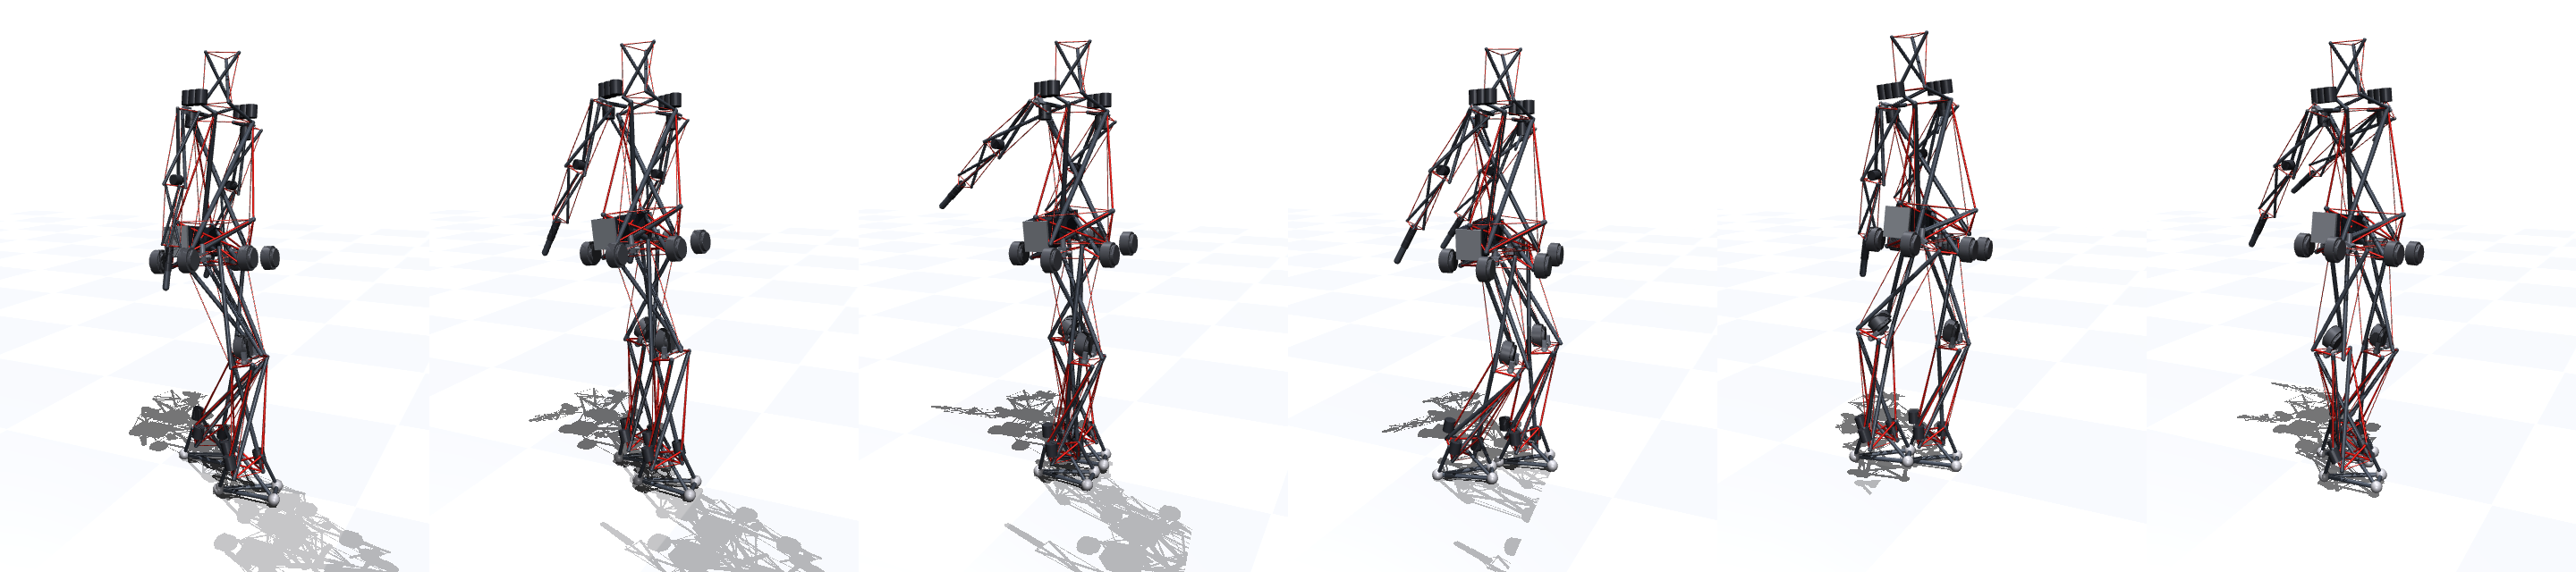
\includegraphics[width=0.99\textwidth]{hybrid_strip.png}
\caption{The hybrid humanoid walking under iLQG in the
stride-lengthened configuration of Sec.~\ref{sec:hybridwalker}
(\agilityV\,m/s, \agilityRate{} of trials); frames advance $7/6$ of a
gait cycle (phase steps a sixth-cycle per frame). Struts are dark, tension members red; the feet and torso are free bodies held only by counter-wound cable interfaces. Arms hold a servo-referenced posture. 1.68\,m, \hybridMass\,kg with both battery packs; see the video attachment.}
\label{fig:sequence}
\end{figure*}

\section{Introduction}
Mass is the binding constraint on humanoid robots. It sets the actuator
torques, which set the motor mass, which sets the battery mass, which sets the
mass again; it sets the energy of every unintended collision; and it governs the hazard a machine of human size poses to the people around it. Conventional humanoids
are chains of rigid links with actuators at the joints, an architecture that
concentrates mass distally, makes collisions stiff, and couples structural
strength to structural weight.

Tensegrity structures \cite{fuller1962patent,snelson1965patent} invert this
logic: disconnected struts float in a network of pre-tensioned cables, every
member is loaded along its axis, and stiffness is a function of prestress
rather than of section. These properties have made tensegrity attractive for
planetary landers and mobile robots
\cite{sabelhaus2015superball,caluwaerts2014design,shah2022tensegrity},
but they have not been carried to a walking machine of human size, and
whether they survive that transition is not something statics can answer.

This paper reports one full iteration of a design loop whose inner step is
model-predictive control: generate a parametric tensegrity kinematics, test
its controllability under tension-only actuation, size actuators and members
from simulated load traces, and ask a receding-horizon iLQG controller
\cite{li2004ilqr,tassa2012synthesis,howell2022mjpc} to balance and walk it.
Every design change is justified by whether it improves the gait. Three
machines of identical anthropometry travel through the paper: \emph{pure
tensegrity}, \emph{fully hinged}, and the \emph{hybrid} between them
that the measurements select.

\textbf{Findings.}
\begin{enumerate}
  \item At 1.68\,m the hybrid masses \hybridMass\,kg, against 30--80\,kg for size-matched humanoids (Table~\ref{tab:compare}); articulation hardware totals \hybridJointHw\,kg because only eight DoF carry bearings.
  \item Because the prestressed network is also the transmission, actuators can be mounted proximally at no additional mechanical cost; doing so measurably improves walk success and speed (Sec.~\ref{sec:evidence}).
  \item Impact attenuation depends on the joint implementation, not on the architecture alone: as built, the tension network \emph{raises} peak ground reaction, while a hinge-free rebuild lowers it by \jointImpactLo--\jointImpactHi\% provided cable stiffness remains series-elastic (Sec.~\ref{sec:jointcell}).
  \item Prestress does not modulate stiffness at rope modulus, where the geometric stiffness term is \jointGeomElasticRope\% of the elastic one; antagonist co-contraction changes endpoint stiffness by $\stiffCoRatio\times$.
  \item Pose-dependent torque authority is the limiting constraint on cable joints: \authShortGaitBom{} of 27 DoF fall below their torque requirement mid-stride, which motivates retaining bearings at hips and knees (Secs.~\ref{sec:authority}, \ref{sec:jointcount}).
\end{enumerate}

\textbf{Contributions.} (i) A 1.68\,m, \hybridMass\,kg \emph{hybrid} humanoid, specified to tube, rope and drive class, walking at \hybridSpeed\,m/s in \hybridRate{} of trials under receding-horizon iLQG (Sec.~\ref{sec:hybridwalker}); (ii) a hinge-free joint geometry --- overlapped cages, counter-wound cable families --- with the result that force closure alone leaves a joint uncontrollable: full wrench closure ($t_6>0$) is required for any balance controller to exist (Sec.~\ref{sec:jointcell}); (iii) a wrench-closure audit and pose-dependent authority bound applied as a design gate over the gait (Sec.~\ref{sec:authority}); (iv) a joint-count study over rigidized variants of one machine, yielding measured trade-offs and an allocation rule (Sec.~\ref{sec:jointcount}); (v) an MPC architecture tracking an analytic gait reference computed inside the cost evaluation, with a pipeline that regenerates every number in this paper from logged runs.

\section{Related Work and Size-Matched Comparison}
\label{sec:related}

\textbf{Tensegrity robotics.} From its artistic origins \cite{fuller1962patent,snelson1965patent} and structural analysis \cite{skelton2009tensegrity}, robotic tensegrity has been demonstrated mainly in rolling or crawling machines: NASA's SUPERball \cite{sabelhaus2015superball,caluwaerts2014design}; the field is surveyed in \cite{shah2022tensegrity}. Control approaches, including learned ones, are covered by the survey; MPC with inverse-statics tension distribution on tensegrity spines \cite{sabelhaus2018spinempc} is the closest precedent for our architecture, though the spines are few-DoF modules loaded quasi-statically. Manipulators \cite{lessard2016manipulator}, modular
cells \cite{zappetti2017modular} and a variable-stiffness spine
\cite{zappetti2020spine} show limb-like assemblies are feasible;
form-finding is reviewed in \cite{tibert2003form};
biotensegrity reads vertebrate joints the same way
\cite{scarr2014biotensegrity}.

\textbf{Tendon-driven and compliant humanoids.} The JSK musculoskeletal line --- Kenshiro \cite{nakanishi2013kenshiro}, Kengoro \cite{asano2017kengoro} --- routes on the order of a hundred muscles over a human-mimetic skeleton with proximal motors and the same unilateral tension constraint we face. What distinguishes the present design is that the tendons \emph{are} the structure: the network applying joint moments also carries the structural tension, so no separate skeleton exists for the muscles to act on. Joint-level compliance in humanoids has its own lineage
through series-elastic actuation \cite{pratt1995series,tsagarakis2013coman};
here series elasticity reappears as a requirement on the tension members
themselves (Sec.~\ref{sec:design}). Soft exosuits \cite{quinlivan2017exosuit}
established that textile load paths carry forces of this magnitude,
motivating our longer-term goal of mounting the structure in standard
apparel.

\textbf{Co-design.} Morphology and control have been optimized jointly by sensitivity analysis through optimal control \cite{ha2018codesign} and by reinforcement learning over design distributions \cite{schaff2019jointly}. We report one manual iteration of such a loop, with a predictive controller as the inner step; nothing here searches design space.

\textbf{MPC for legged robots.} iLQG synthesizes whole-body humanoid behavior from cost functions \cite{tassa2012synthesis,tassa2014control}, and MuJoCo MPC \cite{howell2022mjpc} provides real-time planners. The gait reference draws on Raibert \cite{raibert1986legged} and the capture point \cite{pratt2006capture}. Actuator selection follows Mini Cheetah's quasi-direct-drive approach \cite{katz2019minicheetah}. Torque budgets are from Winter \cite{winter2009biomechanics}.

\begin{table}[tb]
\centering
\caption{Humanoids of comparable stature; mass per unit height compares across slightly different statures. Our two rows are simulated mass budgets, not built machines. The hybrid's 46 DoF include the two free bodies of its tensegrity joints, driven by 30 actuators.}
\label{tab:compare}
\setlength{\tabcolsep}{2.6pt}\footnotesize%
\begin{tabular}{@{}lccccl@{}}
\toprule
robot & m & kg & kg/m & DoF & actuation\\
\midrule
\textbf{this work: hybrid (sim)} & 1.68 & \textbf{20.1} & \textbf{12.0} &
46 & hinge$+$tensegrity\\
this work: hinged (sim) & 1.65 & 27.6 & 16.7 & 27 & tendon, hinged\\
1X NEO Gamma \cite{onex2025neo} & 1.65 & 30 & 18.2 & --- & tendon, soft shell\\
HRP-4 \cite{kaneko2011hrp4} & 1.51 & 39 & 25.8 & 34 & rigid, geared\\
Unitree G1 \cite{unitree2024g1} & 1.32 & 35 & 26.5 & 23 & rigid, quasi-direct\\
Kengoro \cite{asano2017kengoro} & 1.70 & 56 & 32.9 & 114 & musculoskeletal\\
Fourier GR-1 \cite{fourier2023gr1} & 1.65 & 55 & 33.3 & 40 & rigid, geared\\
PAL REEM-C \cite{pal2013reemc} & 1.65 & 80 & 48.5 & 44 & rigid, geared\\
\bottomrule
\end{tabular}
\end{table}

In Table~\ref{tab:compare} the mass spread at fixed stature is nearly threefold --- architecture, not scale, dominates --- and the lightest machines are all tendon-driven with soft shells. The capability gap is equally real: Fourier's GR-1 walks at 1.4\,m/s where the hybrid reaches \hybridSpeed\,m/s in simulation.

\section{The Hybrid Design}
\label{sec:design}
The final design (Fig.~\ref{fig:overview}) is 1.68\,m sole-to-crown and
\hybridMass\,kg, with thigh and shank 0.40\,m (Winter anthropometry
\cite{winter2009biomechanics}) and three joint implementations (Fig.~\ref{fig:joints}). \emph{Hips and knees are bearings} (3-DoF gimbals and clevis pins) because they carry the gait's 40--80\,N\,m through large excursions. Each knee is an alloy-steel clevis pin in a
61802-class bearing pair (\hybridKneeHw\,g); each hip a three-axis gimbal
(\hybridHipHw\,g); all sized with safety factor 2.3 against the measured 1.5\,kN stumble reaction. Articulation hardware totals \hybridJointHw\,kg against the
1.89\,kg of a fully hinged build. \emph{Ankles and waist are tensegrity joints}: each foot is a tri-pad plate (heel and two forefoot
corners, the insertion geometry of the biological ankle
\cite{scarr2014biotensegrity}) whose mast overlaps into the shank cage;
the torso is a free body whose cage nests into the pelvis girdle. Both are held only by the counter-wound cable interfaces of Sec.~\ref{sec:jointcell}: twelve cables each, no bearing, and force and wrench closure by construction. Cables at a hinge-free joint act at the cage radius rather
than through a $\sim$37\,mm effective arm, so the same moment costs an
order of magnitude less tension: 0.165\,kg XM540-class drives replace the
0.96\,kg units a hinged ankle needs. 
Each arm has seven DoF: a shoulder gimbal, an elbow, and a three-axis wrist, with all drives massed and drawn. While walking, only the two swing DoF per arm are planned; the rest hold position on servo stiffness, modeled explicitly as joint stiffness. The neck is rigid in this iteration: the head cage mounts to the torso on a fixed strut tripod, with no articulation. Two 2.5\,kg battery packs ride posterior pelvis rails below the waist joint.

Every segment is a Snelson 3-strut prism cell at the \emph{form-found} equilibrium twist. Released free-floating in zero gravity, the cell converges to $29.8^\circ\pm0.4^\circ$, and that measured twist, not the textbook $30^\circ$, generates all cages.

Two earlier variants of the same anthropometry bound the design space and
recur as comparison points: the \emph{fully hinged} 27-DoF machine (every
joint a bearing, tendon-driven --- the configuration most humanoids use) and
the \emph{pure tensegrity} machine with no bearings
(Sec.~\ref{sec:jointcell}). Joint torque limits come from human walking
moments scaled to robot mass at safety factor $\approx$2 (hip pitch and knee
80\,N\,m, ankle 70\,N\,m, shoulder 30\,N\,m on the hinged machine, 15\,N\,m
XM540-class on the hybrid).

\begin{figure}[tb]
\centering
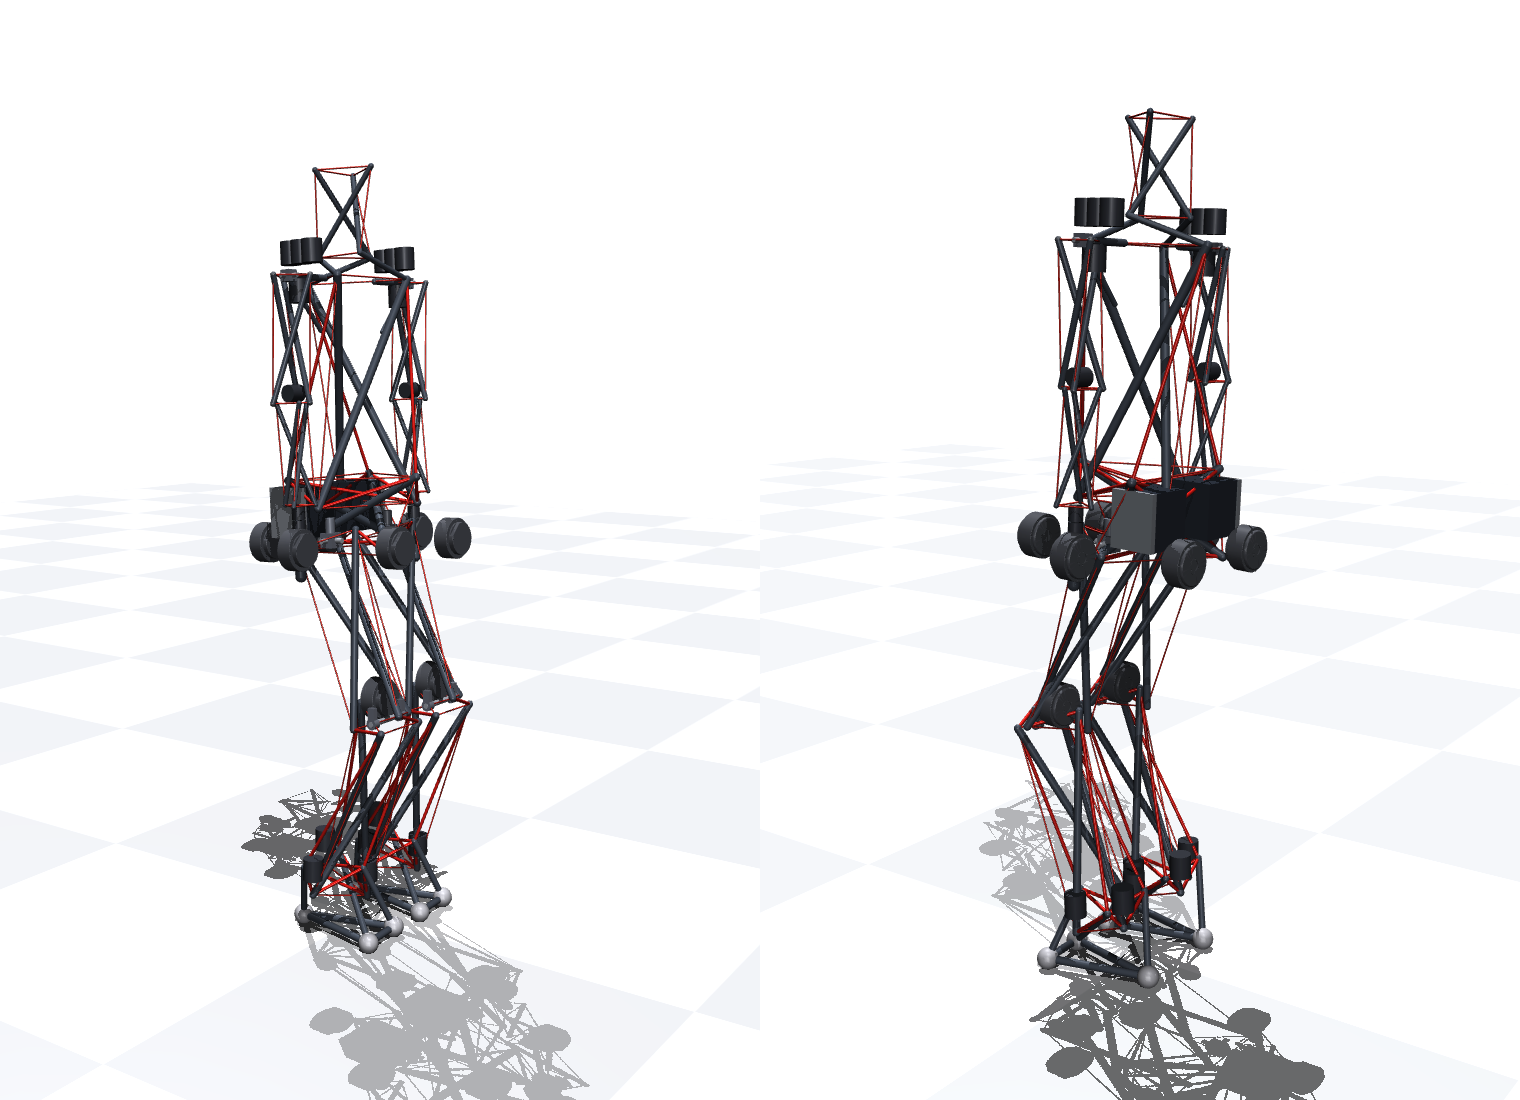
\includegraphics[width=0.68\linewidth]{hybrid_overview.png}
\caption{The hybrid humanoid, front and rear. Every segment is a prism cage; AK70-class hip drives ring the pelvis girdle, battery packs ride posterior rails, XM540-class drives sit on shank rings and torso. Red members are cables: cell cables triangulating each cage, counter-wound joint cables at ankles and waist.}
\label{fig:overview}
\end{figure}

\begin{figure}[tb]
\centering
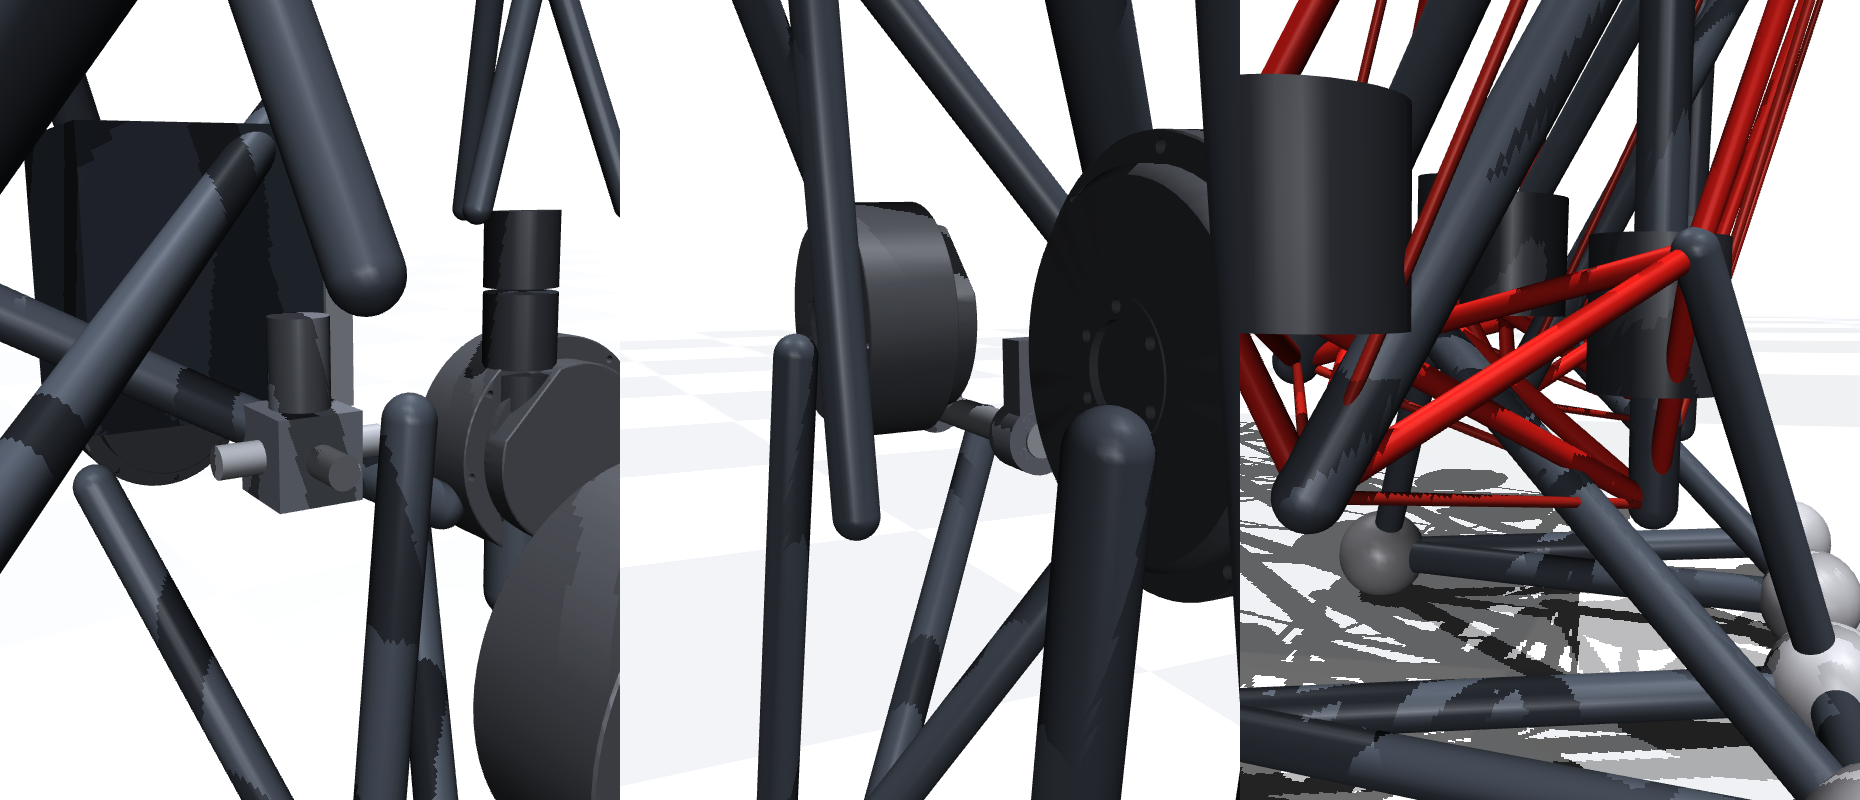
\includegraphics[width=0.99\linewidth,trim=0 40 0 0,clip]{hybrid_joints.png}
\caption{The three joint types, left to right: hip --- three-axis
gimbal: yaw pivot descending from the girdle, cross block, roll and pitch
axles; knee --- drive disc on the thigh cuff, clevis lugs and steel
cross-pin between the cages; ankle --- no bearing: the foot's mast reaches
into the shank cage and twelve counter-wound cables (red) carry the joint.
Cell cables are hidden in the first two panels for clarity.}
\label{fig:joints}
\end{figure}

\textbf{Member specification.} Since the structural argument for tensegrity rests on the members, each is dimensioned explicitly from the simulated load cases rather than covered by a bulk mass allowance.
\numStruts{} CFRP tubes, 12--20\,mm outer diameter: the governing axial load is the ground reaction entering a cage through its joint (\strutLoadStumble\,N per strut at a 0.1\,m stumble), not cable tension. Even so, Euler sizing at safety factor 2 puts \emph{every} strut at the minimum manufacturable wall (\strutWall\,mm; worst margin $\strutWorstMargin\times$). The compression network is therefore manufacturability-limited, not load-limited, at \strutTubeMass\,kg of tube plus \strutFittingMass\,kg of fittings. Tendons are 12-strand UHMWPE sized from the larger of the gait's 99th-percentile tension and the loop requirement $\tau_{\max}/r_{\mathrm{eff}}$ (4\,mm legs and waist, 2.5\,mm shoulders, 1\,mm cell cables; worst RMS utilization \ropeUtilRms\%). The rope itself is \ropeMass\,kg, but its
\numCableEnds{} terminations mass \termMass\,kg and the \nodeCount{} node
clusters \nodeMass\,kg --- a network of this kind is priced by its
interface count, not its cable count.

\textbf{Cable stiffness: model versus hardware.} Specified rope runs \kRopeMin--\kRopeMax\,MN/m; the simulation models cables at \kModelMin--\kModelMax\,N/m. A deliberate series-elastic element of \kSeriesMin--\kSeriesMax\,kN/m \cite{pratt1995series} is required for prestress to be practical to set during assembly, and is what the transmission analysis assumes; the model remains $\sim$\stiffGapSeries$\times$ softer than even that element --- the largest modeling gap in this work (Sec.~\ref{sec:discussion}).

\begin{table}[tb]
\centering
\caption{Mass budget of the hybrid. Every drive is mounted proximally to the
joint it serves; the two tensegrity joints carry no bearings.}
\label{tab:mass}
\setlength{\tabcolsep}{4pt}%
\begin{tabular}{@{}lccl@{}}
\toprule
item & $n$ & kg & where\\
\midrule
hip drives, AK70-class & 6 & 3.1 & pelvis girdle\\
knee drives, AK70-class & 2 & 1.0 & thigh cuffs\\
ankle tension drives, XM540 & 6 & 1.0 & shank rings\\
waist tension drives, XM540 & 6 & 1.0 & torso ring\\
arm drives, XM540/XM430 & 14 & 1.7 & torso + arm\\
articulation hardware (gimbals, clevises) & & 0.8 & hips, knees\\
battery packs, hot-swappable & 2 & 5.0 & pelvis rails\\
compute + power & & 0.5 & pelvis\\
structure: cages, cables, feet, masts & & 6.0 & distributed\\
\midrule
total & & 20.1 & \\
\bottomrule
\end{tabular}
\end{table}

\section{Modelling, Authority, and Control}
\label{sec:authority}
The machines are modeled in MuJoCo \cite{todorov2012mujoco} by a parametric generator that produces, from one description of the node geometry, a \emph{joint-torque} model (motors
at the hinges; the planner's model) and a \emph{cable-driven} model
(\numActuatable{} tension-only actuators). Two implementation points matter beyond standard MuJoCo model files. \emph{Cables must be tension-only}: a MuJoCo tendon
with a single spring length pushes when short, making every ``cable''
secretly a strut; all cables therefore use a deadband spring,
$F=k\max(0,\ell-\ell_0)$ with $\ell_0$ set by the prestress fraction and
recomputed from the compiled model so wrapped cables carry the intended
prestress.

\emph{Long-axis rotations need capstan drums}: a cable helixed
around a limb has a 16--25\,mm moment arm about the limb axis, so yaw DoF
carry a coaxial drum (35--55\,mm) that fixes the arm independently of cage
geometry. Four checks run automatically after every geometry change: all \numEndpoints{}
cable endpoints coincide with strut tips (no cables ending in mid-air), the
authority analysis below, a scripted balance test, and the same balance by
pure tension distribution on the cable model at 250\,Hz.

\textbf{Cable authority.} With tension-only
actuation the achievable torque about DoF $j$ is bounded by
\begin{equation}
  \tau_j^{+} = \sum_c \max(0, M_{jc})\,\Fmax_c,\qquad
  \tau_j^{-} = \sum_c \min(0, M_{jc})\,\Fmax_c,
  \label{eq:authority}
\end{equation}
where $M_{jc}=\partial\ell_c/\partial q_j$ is the moment arm of cable $c$
about joint $j$ and $\Fmax_c$ its tension limit --- the per-DoF projection of
the wrench-feasibility condition of the cable-driven parallel robot
literature \cite{bosscher2004wrench,gouttefarde2007wfw};
we claim no novelty for the bound, only for applying it to a legged machine as a requirement \emph{over the whole trajectory} rather than at one pose. Used this way it caught three errors:
hip yaw and wrist had exactly zero authority in one direction because all
cable families wound with the same handedness (opposite-handed winding is
required for bidirectional yaw --- a rule that returns, generalized, in
Sec.~\ref{sec:jointcell}); shoulder roll had $0.15\times$ the required
torque from a misplaced socket; and ankle cables saturated during push
recovery until the foot nodes moved to heel/forefoot positions. As a guarantee it is far weaker than the assembly-pose number suggests (Table~\ref{tab:authority}): at assembly, all 27 DoF are bidirectional (worst margin $\authHomeAll\times$); at logged gait poses, \authShortGaitAll{} of 27 fall below their torque limit (hip pitch $\authGaitHip\times$, knee $\authGaitKnee\times$), and the \numDrivenCables{}-cable, \numMotors-motor bill of materials leaves \authShortGaitBom{} of 27 short. The exact
zeros in Table~\ref{tab:authority} are the capstan drums: wrap disengages
at some wrist and shoulder angles, and authority there is not merely small
but absent. Covering
80\,N\,m at the 1.5\,kN cable limit needs $r_{\mathrm{eff}}\ge\rNeedHip$\,mm;
the cage offers \rHaveHip\,mm at hip pitch. This shortfall is the quantitative reason the hybrid keeps bearings at hips and knees. The moment arms collapse mid-stride, and adding motors does not help: a second cable of the same family loses its arm at the same poses.

\begin{table}[tb]
\centering
\caption{Cable authority (Eq.~\ref{eq:authority}) on the fully hinged
variant depends on where it is evaluated and which cables a motor can reach.
Entries: DoF short of their torque limit, and worst margin over 27 DoF.}
\label{tab:authority}
\begin{tabular}{llcc}
\toprule
configuration & actuation set & DoF short & worst margin\\
\midrule
assembly pose & all cables & \authShortHomeAll{}/27 & $\authHomeAll\times$\\
gait poses    & all cables & \authShortGaitAll{}/27 & $\authGaitAll\times$\\
assembly pose & \numMotors{} loops & \authShortHomeBom{}/27 & $\authHomeBom\times$\\
gait poses    & \numMotors{} loops & \authShortGaitBom{}/27 & $\authGaitBom\times$\\
\bottomrule
\end{tabular}
\end{table}

\textbf{Predictive control.} The controller is MJPC's asynchronous iLQG \cite{howell2022mjpc,tassa2012synthesis} with control limits \cite{tassa2014control}: horizon 0.6\,s, planning timestep 20\,ms, plant at 4\,ms. Hand-designed cost terms alone produced only stepping in place; two of those terms actively opposed walking (a pelvis line term forbids the weight shift that unloads a foot; a permanent capture-point term is wrong in single support). The remedy is
an \emph{analytic gait reference computed inside the cost evaluation}: gait phase is a function of time alone, and the pelvis tracks a lateral sway timed so that weight is over each stance foot just before the other lifts. Stance feet slide back while swing feet return with sinusoidal clearance, half a cycle apart. The swing landing point is biased by center-of-mass velocity error in the manner of Raibert \cite{raibert1986legged} and the capture point \cite{pratt2006capture}; this bias is what makes stepping stabilizing. Foot targets become leg-joint references by analytic flat-foot inverse kinematics, with posture referenced to a bent-knee walk-ready pose.

\textbf{Walking results, fully hinged variant.} This machine validates the pipeline and produces the load traces used for dimensioning: \walkSpeed$\pm$%
\walkSpeedSd\,m/s in \walkRate{} of ten trials, longest run 6\,m in 29\,s,
at \realtimeFactor$\times$ real time on a laptop CPU. Cost of transport is \walkCot. Drives are dimensioned from the traces: force bandwidth through series compliance
$f_{\mathrm{bw}}=\frac{1}{2\pi}\sqrt{k_{\mathrm{ser}}/m_{\mathrm{eff}}}$
with $m_{\mathrm{eff}}=I_rG^2/r^2$ splits the transmissions by what dominates each joint: spools where stroke dominates (hips, knees, waist), lever arms where bandwidth dominates (ankles, 46\,Hz), and drums where the rotation axis itself is the problem (yaw). The resulting
\numMotors-motor bill of materials, however, \emph{does not meet its own
torque specification}: a single loop delivers \singleLoopHip\,N\,m at hip
pitch against 80 required, and Table~\ref{tab:authority} shows the shortfall
widening over the gait. The fix is geometric (enlarge
$r_{\mathrm{eff}}$), not more motors.

\section{Evidence on the Fully Hinged Variant}
\label{sec:evidence}
Five experiments run against a \emph{rigid-equivalent baseline} --- the same
27-DoF model with the tension network removed --- with actuation held
constant, so only the structural paradigm varies
(Table~\ref{tab:experiments}).

\textbf{E1, impact.} In matched-pair drops of 0.05--1\,m the tension network \emph{raises} peak ground reaction at every height: +\eOneDeltaPassiveStumble\% limp at 0.1\,m, and \physOneLimpTen--\physOneLimpHundred\% at physical cable stiffness. A bearing puts the elastic network in parallel with a stiff path, and impulses take the stiff path. \textbf{E2, stiffness.} Under a \stiffProbe\,mN differential endpoint probe, cables raise lateral stiffness $\stiffCablesRatio\times$ by their presence alone, but assembly prestress swept $0$--$5\times$ moves it only within \stiffPreLo--\stiffPreHi\,N/m: prestress does not modulate stiffness at rope modulus (Sec.~\ref{sec:jointcell} isolates why). Differential tension does --- shoulder co-contraction moves \stiffCoLo$\to$\stiffCoHi\,N/m ($\stiffCoRatio\times$) with no added hardware. \textbf{E3, degradation.}
All \eThreeSinglesOk/\eThreeSinglesN{} single cable cuts and every random
loss up to $k=8$ survive standing plus a push; an adversary selecting
against the authority margin kills at $k=8$. No single cable is structural,
where one failed gearbox in a rigid robot is one dead joint. \textbf{E4,
proximal mass.} Moving motor masses to the joints they drive, totals
identical, degrades walking from \walkRate{} to \distalRate{} and \walkSpeed{} to \distalSpeed\,m/s, quantifying the benefit of proximal mounting under tendon transmission. \textbf{E5, tendon realisability.} Mapping logged walking torques
through the bounded tension distribution: the network reproduces demanded
torques exactly for most of the stride (median residual
$<10^{-3}$\,N\,m) with concentrated failures --- a cable pinned at its
1.5\,kN limit in \tensSatPct\% of states, leaving up to
\tensResidTwelve\,N\,m undelivered; the gait asks for \tensNeeded\,N peak
tension, $1.6\times$ the specified rating. Re-planning \emph{inside} the
achievable envelope separates topology from actuation: a gait exists for
the full network (\eSixtendonallRate) but not for the bill of materials
(\eSixtendonbomRate). The topology can support a gait; the actuation set as
specified cannot deliver one. Its capability envelope (65\% speed tracking to 0.29\,m/s; trunk payload flat to 20\,kg) appears as the grey references in Fig.~\ref{fig:sweeps}.

\begin{table}[tb]
\centering
\caption{Experiment summary, all on the fully hinged variant against the
rigid-equivalent baseline, actuation held constant; walking conditions
$n=10$.}
\label{tab:experiments}
\setlength{\tabcolsep}{3pt}\footnotesize%
\begin{tabular}{@{}llp{4.6cm}@{}}
\toprule
id & property & result\\
\midrule
E1 & impact tolerance & network raises peak reaction at every drop height
(\physOneLimpTen--\physOneLimpHundred\% at physical stiffness)\\
E2 & stiffness on demand & assembly prestress: no effect
(\stiffPreLo--\stiffPreHi\,N/m); co-contraction: $\stiffCoRatio\times$\\
E3 & graceful degradation & all singles and random $k\le8$ cuts survive;
adversarial $k{=}8$ fails\\
E4 & proximal mass & distal motors: \distalRate{} vs \walkRate{} walks,
\distalSpeed{} vs \walkSpeed\,m/s\\
E5 & tendon realisability & \authShortGaitBom{}/27 DoF short over gait;
gait exists for full network, not for BOM\\
\bottomrule
\end{tabular}
\end{table}

\section{The Hinge-Free Joint}
\label{sec:jointcell}
Is the fully hinged variant's failure to deliver impact tolerance and
prestress-tunable stiffness a fact about tensegrity, or about its hinges?
An audit answers the prior question first: that machine's joints \emph{are}
bearings --- every articulated interface fixes all three relative
translations, and the wrench-closure LP (closure iff
$\max\{t: W\lambda=0,\ \lambda\ge t\mathbf{1}\}>0$ for the matrix
$W$ of unit-tension cable wrenches \cite{bosscher2004wrench,gouttefarde2007wfw})
reports \wcThree/\wcTotal{} joints able to resist even pure forces by
cable alone: every crossing cable pulls the segments together, and nothing
resists approach. Removing the hinges confirms it dynamically --- the robot
telescopes and collapses within two seconds.

\textbf{Force closure requires overlap; wrench closure requires counter-winding.} In a tensegrity tower, stages \emph{overlap}: the distal ring sits inside the proximal cage, giving the interface a downward as well as an upward cable family. On an isolated two-cage testbed (fixed proximal cage, three floating distal struts, 1\,kg payload), force closure appears from \jointOverlapFrac$H$ of overlap and the joint carries load. Force
closure is not enough. An earlier version of this analysis read the
wrench-closure margin $t_6=0$ as benign; controlling the joint exposed the
error. $t_6=0$ means the cable set has \emph{no self-stress}: no co-contraction state and zero moment authority about some axis. Tension-only actuators can then only add load to an equilibrium, never oppose a disturbance, so no balance controller can exist. A controllable joint needs $t_6>0$, with
actuators choosing how much moment to exert, including none. The single
cross family winds one way and cannot do it; adding the \emph{counter-wound mirror family} closes the wrench set at the same cable count. This is the opposite-handedness rule required at the yaw drums, not previously recognized as general. With the counter-wound pair the joint carries load, holds
$\ge$1.3\,kN of co-contraction authority, and a chain of them stands
passively.

\textbf{Impact attenuation at the hinge-free joint.} Dropping the testbed
against a mass-matched control whose distal cage rides a ball joint, peak
ground reaction falls from \jointImpactPinFive{} to
\jointImpactCableFive\,N at 0.05\,m, \jointImpactPinTen{} to
\jointImpactCableTen\,N at 0.10\,m, and \jointImpactPinTwenty{} to
\jointImpactCableTwenty\,N at 0.20\,m --- attenuation of
\jointImpactLo--\jointImpactHi\% at every height, where the hinged humanoid
\emph{raised} it (E1). Remove the bearing and the elastic network is in series with the load rather than parallel to a stiff path, the arrangement the tensegrity-lander results rely on \cite{sabelhaus2015superball}. The attenuation belongs to the series
compliance that the topology puts into the load path, not to the topology
alone: repeating the drops at $10\times$ cable stiffness (400\,kN/m,
toward bare rope) \emph{inverts} the comparison, the cable joint landing
\stiffSensTenLo{} to \stiffSensTenHi\% harder than the pin joint.
Hinge-free geometry and series-elastic cables buy impact tolerance
jointly; neither suffices alone. \textbf{Prestress-tunable stiffness remains absent}, and the mechanism is a materials condition rather than a topology property:
tangent stiffness is an elastic term $\mathcal{O}(EA/L)$ plus a geometric
term $\mathcal{O}(T/L)$, and prestress tunes stiffness only when they are
comparable. At the rope modulus this design specifies the geometric term is
\jointGeomElasticRope\% of the elastic one (hinge or no hinge); the
cell-scale demonstrations that motivated the claim used cables three orders
of magnitude softer. Variable stiffness must be budgeted as an actuation
cost (co-contraction, E2), not an assembly parameter.

\textbf{Composition into a complete assembly.} Generating the entire machine as a graph of
overlapping cells --- no bearings, nothing touching --- stands
(\cgStruts{} struts, \cgCables{} cables; limb chains droop
$\approx$\cellChainPer\,mm/cell). But junctions cannot be cells (a prism
hosts two interfaces; a pelvis needs three), so pelvis and torso become
rigid strut clusters, and carrying the 22\,kg of motors and batteries
takes \cgPreNeeded\,N of prestress per cable --- an order of magnitude
beyond the single-joint level, forcing 3\,kN-rated cell cables. The pure machine exists structurally, at a quantified cost; what does not exist is a controller for its \cgDof{} floating DoF (Sec.~\ref{sec:discussion}).

\section{The Hybrid Walker}
\label{sec:hybridwalker}
The prescription that emerges --- bearings where torque requirements dominate, tensegrity where compliance dominates --- is the hybrid of Sec.~\ref{sec:design}. This section reports its walking performance and the whole-machine effects of its two tensegrity joints.

\textbf{Gait synthesis.} The controller is the analytic-reference iLQG task with the ankle posture rows deleted. With the ankle cables \emph{passive}, every configuration fails identically: the planner does not lift the swing foot. Without ankle actuation there is no center-of-pressure control, so a foot can be unloaded only by whole-body sway, and lifting a loaded foot would lift the robot. Welding the feet to the shanks walks immediately at 0.18\,m/s, isolating the cause. Giving the
planner tension actuators on two of the four ankle cable families (twelve
controls, tension-only) recovers walking at \hybridSpeed\,m/s in
\hybridRate{} of trials --- at a running cost \emph{below} the welded
control, because the planner exploits the compliance it now commands: one
family lifts the hanging foot for swing clearance, the other pitches the
toe, differential tension steers the landing. With actuated cables the tensegrity joint therefore constitutes the better-performing ankle in this comparison. Actuator utilization confirms the sizing: hip and knee motors average \hybridJointDuty\% of their limits, ankle actuators \hybridAnkleDuty\% with \hybridAnklePeak\,N peaks at foot lift; the 46\,Hz bandwidth demand of the hinged ankle disappears, absorbed by cable compliance. The torso rides the waist cables within $\pm2^\circ$, and pulling one battery mid-stance leaves the gait intact.

\begin{figure*}[tb]
\centering
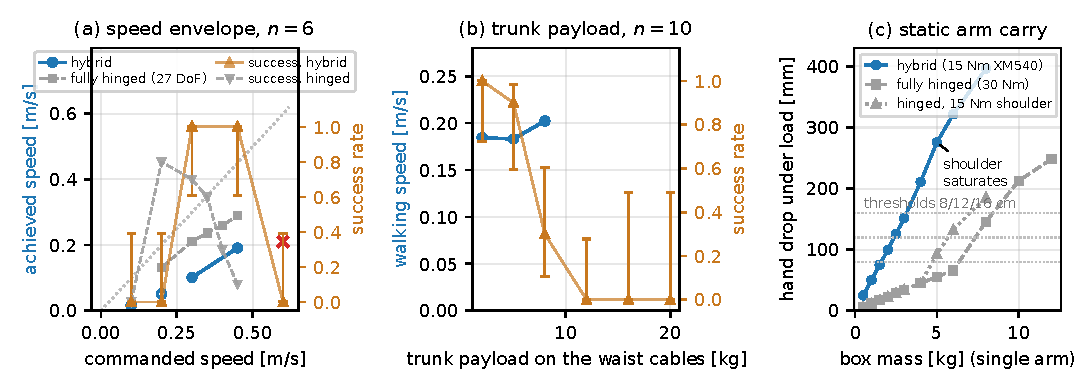
\includegraphics[width=0.98\textwidth]{sweeps.pdf}
\caption{Capability sweeps on the hybrid; error bars are Wilson 95\%
intervals on the success rate. (a) Achieved speed and success rate vs.\ commanded speed ($n=6$), fully hinged envelope in grey; 0.10--0.20\,m/s commands are upright but undertracking, not falls. (b) Trunk payload
carried above the tensegrity waist ($n=10$ to 12\,kg, $n=4$ beyond):
reliable at 2\,kg, degrading through 8\,kg, gone by 12\,kg for a centerd load, where the hinged machine's rigid trunk was flat to 20\,kg (a placement intervention restores 10\,kg at \payTenRate; see text). (c) Static single-arm carry, matched protocol (pelvis welded, identical pose and gains): hand drop vs.\ box mass, thresholds dotted. The hybrid is sag-limited (\carryHybSlope\,mm/kg; hold moves \carryHybEight$\to$\carryHybSixteen\,kg with the threshold), the hinged machine motor-limited (\carryHinSlope\,mm/kg until its 30\,N\,m shoulder saturates; \carryHinEight$\to$\carryHinSixteen\,kg).}
\label{fig:sweeps}
\end{figure*}

\textbf{Capability envelope} (Fig.~\ref{fig:sweeps}). \emph{Speed:} the hybrid has a reliable command band rather than a smooth degradation: \hsSpdThirtyRate{} at a commanded 0.30\,m/s (\hsSpdThirtyV\,m/s achieved), \hsSpdFortyFiveRate{} at 0.45 (\hsSpdFortyFiveV), and falls in every trial at 0.60. Below the band it does not fall but undertracks (0.02--0.05\,m/s at 0.10--0.20 commanded): the sway-and-step reference has a minimum viable tempo. Gait-parameter retuning then extends the band. Lengthening the stride (cadence 1.1$\to$0.8\,Hz at the same command) and raising the swing-height reference to 0.24\,m with doubled cartesian tracking weight reaches \agilityV\,m/s at \agilityRate{}, with measured swing clearance of \gaitClr\,mm --- the configuration of Fig.~\ref{fig:sequence}. The swing-height reference must be commanded at roughly three times the desired clearance: clearance tracks the reference (11, 18, \gaitClr\,mm at references of 0.08, 0.16, 0.24\,m) while extending the planning horizon has no effect. Raising the speed command to 0.55 at the original cadence reaches \agilityFastV\,m/s at only \agilityFastRate. The remaining panels of Fig.~\ref{fig:sweeps} are measured at the pre-retune configuration. Tracking is the larger difference,
$\approx$42\% of command against the hinged 65\%: part of every push-off is stored in the elastic network rather than delivered to the ground, a speed cost of compliance that Sec.~\ref{sec:jointcount} measures joint by joint. \emph{Trunk payload:}
boxes on the torso ride \emph{above} the tensegrity waist, so every added
kilogram loads the twelve waist cables. The envelope is correspondingly
smaller: \hsPayTwoRate{} at 2\,kg (speed within noise of unloaded),
\hsPayFiveRate{} at 5, \hsPayEightRate{} at 8, \hsPayTwelveRate{} at
12\,kg --- against flat-to-20\,kg on the rigid trunk. At 12\,kg every trial falls within the first strides, seven of ten \emph{backward} --- the loaded waist pitches the trunk aft faster than the planner corrects within its horizon. The hinged machine's payload was tendon-limited at the leg; the hybrid's is limited by pitch stability at the compliant waist. An intervention study at 10\,kg identifies payload placement as the effective lever: with the load's center of mass 4\,cm anterior of the waist axis (cancelling the static moment of the posterior battery packs) and the speed command reduced to 0.40\,m/s, the machine carries 10\,kg at \payTenRate{} and \payTenV\,m/s. Waist stiffening and torso-height corrections did not help: the constraint is dynamic pitch balance, not static capacity.
\emph{Arm carry:} under one protocol on both machines (pelvis welded,
same pose and gains; failure = hand drop from the settled unloaded
position), the hybrid holds \carryHybTwelve\,kg at a 12\,cm threshold
where the hinged machine holds \carryHinTwelve\,kg. The failure modes
differ in kind: the hybrid's limit moves
\carryHybEight$\to$\carryHybSixteen\,kg as the threshold moves
8$\to$16\,cm (sag-limited: \carryHybSlope\,mm/kg through seven
servo-compliant joints, shoulder at 71\% at failure), while the hinged
machine's barely moves, \carryHinEight$\to$\carryHinSixteen\,kg
(motor-limited: its stiff chain sags \carryHinSlope\,mm/kg until the
30\,N\,m shoulder saturates). Halving the drive class costs two thirds of the carry rather than half (compliance compounds the torque deficit), and the carry loads a path the hinged machine lacked: the busiest waist cable rises from 52 to 88\,N under a 2\,kg hold.

\section{How Many Joints Does a Humanoid Need?}
\label{sec:jointcount}
The hybrid fixes one point on an axis from no bearings to a bearing at
every DoF. Table~\ref{tab:jointcount} walks the axis with variants of the
\emph{same} machine --- identical masses, drives, anthropometry ---
differing only in which joints are bearings, run under the hybrid's final controller configuration, bracketed by the two endpoints with their own tuning.

\begin{table}[tb]
\centering
\caption{The joint-count axis. Middle rows are variants of the hybrid under its final controller ($n=5$); endpoints carry their own tuning.
``T-joints'' counts tensegrity (bearing-free) joints. The impact figures
are from the ankle-joint testbed (Sec.~\ref{sec:jointcell}) and E1
respectively.}
\label{tab:jointcount}
\setlength{\tabcolsep}{2.6pt}\footnotesize%
\begin{tabular}{@{}lccccl@{}}
\toprule
variant & brgs & T-jts & walks & m/s & note\\
\midrule
pure tensegrity & 0 & all & --- & --- & stands only; no planner\\
\textbf{hybrid (design)} & 0.8\,kg & 3 & \textbf{\hybridRate} &
\hybridSpeed & impact $-$27..32\% (ankle)\\
\;+ rigid waist & 0.8\,kg & 2 & \jcRWaistRate$^\dagger$ & --- &
tuning mismatch\\
\;+ rigid ankles & 0.8\,kg & 1 & \jcRAnkleRate & \jcRAnkleV & \\
\;+ both rigid & 0.8\,kg & 0 & \jcRBothRate & \jcRBothV & \\
fully hinged (27\,DoF) & 1.9\,kg & 0 & \walkRate$^\ddagger$ & \walkSpeed &
impacts $+$14..154\% (E1)\\
\bottomrule
\multicolumn{6}{@{}p{8.2cm}@{}}{\footnotesize $^\dagger$fails under the
hybrid's tuning; retuned --- one parameter, the torso height target,
1.20$\to$\jcRWaistTunedTorso{} (the welded torso stands taller than the
cable-mounted one settles) --- the same joint set with the same arms walks
\jcRWaistTunedRate{} at \jcRWaistTunedV\,m/s. $^\ddagger$own tuning at
its 0.30\,m/s operating point; its envelope edge is 0.29\,m/s at a 0.45
command (Fig.~\ref{fig:sweeps}a). Source of the load traces and E1--E5.}
\end{tabular}
\end{table}

\textbf{The case for retaining bearings.} \emph{Load path}: without overlap and counter-winding a hinge-free joint is not a structure. \emph{Torque}: a bearing delivers full torque at every angle; a cable joint's authority collapses mid-stride (Table~\ref{tab:authority}). \emph{Planning}, in practice the dominant layer: every bearing removes three to five DoF from the state a predictive controller reasons over. The hybrid's planner handles 46 DoF at $0.3\times$ real time; the pure machine has \cgDof, and no controller in this work or, to our knowledge, elsewhere stabilizes it. Bearings at hips and knees make the
machine \emph{plannable} and its gait torques available at every pose.

\textbf{Consequences of replacing bearings with cable interfaces.} Replacing a bearing with a cable interface provides impact attenuation ($-27$..$32\%$ at the ankle testbed; $\pm2^\circ$ torso compliance), an order of magnitude lighter actuation (0.165 vs.\ 0.96\,kg drives at cage-radius moment arms), graceful degradation (no single cable is structural), and robustness to mass change (the battery-removal test). The corresponding costs are
\emph{speed} (rigidizing raises gait speed monotonically, $\hybridSpeed\rightarrow\jcRAnkleV\rightarrow\jcRBothV$\,m/s under one controller, because part of each push-off is stored elastically), \emph{planner
load} (each cable joint returns six DoF; $0.3\times$ real time vs.\ the
hinged machine's $0.6\times$), \emph{payload} (the waist ceiling of
Fig.~\ref{fig:sweeps}b), and \emph{tuning fragility}, most visible in Table~\ref{tab:jointcount}: the gait tuned for the compliant waist
fails outright (\jcRWaistRate) when that joint is rigidized. Joint compliance is not a drop-in property; controller and structure must be tuned jointly.

\textbf{Allocation rule.} Place bearings where the gait's torque requirements concentrate, and cable interfaces where impacts enter the structure. Hips and knees carry the largest,
most pose-varied torques and no first impact: bearings. Ankles meet the
ground first and need an order of magnitude less moment: cables. The waist
is the marginal case: a cable waist provides torso compliance at a cost in speed, payload and tuning effort. The hybrid's split saves 1.1\,kg of bearings over the fully hinged machine, recovers the impact attenuation and degradation tolerance that machine lacks, and remains controllable.

\textbf{The biological counterexample.} The human body appears to contradict this rule. Though jointed at every limb, biotensegrity reads the skeleton as a continuous tension network whose articular surfaces are held by ligament and muscle tension rather than axles \cite{scarr2014biotensegrity}: the joint sits inside the tensegrity. The biological knee addresses both problems that led this design to bearings: the patella enlarges the extensor moment arm where the cages fall short of $r_{\mathrm{eff}}\ge\rNeedHip$\,mm, and graded co-contraction supplies closure and disturbance rejection. Biology adds the controller for the high-dimensional compliant state that our planner does not handle. The rule is thus a statement about present-day drives and planners; the human body indicates the all-tensegrity endpoint is reachable with sufficient control.

\section{Discussion and Open Questions}
\label{sec:discussion}
\textbf{Measured benefits of the tensegrity paradigm.} The paradigm provides mass efficiency (compression network at minimum wall, \strutSpecMass\,kg), a transmission at no additional mechanical cost (the prestressed network \emph{is} the transmission; E4), redundancy (E3), impact attenuation in hinge-free form only (Sec.~\ref{sec:jointcell}), hence tensegrity at ankles and waist, and variable stiffness as a co-contraction cost rather than an assembly parameter. It does not provide pose-independent torque, which binds hardest at hips and knees.

\textbf{Realizability.} A simulation-only study must state how its claims can be tested in hardware. Every member and drive is a catalog part with a stated rating, and the machine decomposes into bench-scale units. Table~\ref{tab:ladder} attaches to each unit a prediction simulated under the conditions the bench would apply; discrepancies then localize at components rather than inside a 46-DoF machine. Geometric predictions (twist, closure, moment arms) do not depend on the largest model gap, cable stiffness; the compliance predictions do, and sit early in the ladder where refitting is cheapest. Each stage tests the simulation before the next is built.

\begin{table}[tb]
\centering
\caption{Staged validation ladder: bench-scale units in build order, each with the simulated prediction a bench test would check. The arm row uses the protocol of Fig.~\ref{fig:sweeps}c.}
\label{tab:ladder}
\setlength{\tabcolsep}{2.5pt}\footnotesize%
\begin{tabular}{@{}llp{2.7cm}@{}}
\toprule
stage (unit) & quantity & prediction\\
\midrule
cell (3 tubes, 9 cables) & twist; stiffness vs.\ prestress &
$29.8^\circ\pm0.4^\circ$; flat\\
ankle (plate, mast, & arms; N\,m/100\,N &
\benchAnkleArmA{}--\benchAnkleArmB\,mm; \benchAnkleMoment\\
\;12 cables, 2 drives) & drop at 40 / 400\,kN/m & $-$27..32\% /
inverts\\
knee pin, hip gimbal & 1.5\,kN proof load & SF\,2.3, no yield\\
arm (7 DoF, mount) & loaded sag; first mode & \carryHybSlope\,mm/kg;
3.6\,Hz\\
waist (torso on pelvis) & sink; capacity &
\benchWaistSink\,mm/100\,N; holds 200, fails 300\,N\\
leg (guided-pelvis jig) & cable T vs.\ load &
\benchLegT$\to$\benchLegTTwo\,N at $+$200\,N\\
machine & stand, then walk & \agilityRate{} at \agilityV\,m/s\\
\bottomrule
\end{tabular}
\end{table}

\textbf{Limitations.} Everything is simulated: no tendon friction, hysteresis, creep or cable mass, and cables $\sim$\stiffGapSeries$\times$ softer than the specified series-elastic element. The joint-scale impact result is stiffness-swept (it inverts at $10\times$); the whole-machine compliance numbers are not and are the most exposed. Cost of transport (\walkCot) is 5--15$\times$ that of comparable machines and the planner runs at $0.3\times$ real time. Mass parity against an equivalent rigid frame, contact safety, and fatigue remain untested.

\textbf{Open questions.} \emph{Can a hinge-free humanoid be planned for?} The structure exists (Sec.~\ref{sec:jointcell}) and biology indicates the control problem is solvable; whether by predictive control over a $\sim$210-DoF state or a reduced cell-as-joint model remains open. \emph{Which design variables dominate the next iteration?} Moment-arm geometry (Eq.~\eqref{eq:authority} as a workspace constraint) and tension-member softness, whose trade shows a cliff between 40 and 400\,kN/m.

\section{Conclusion}
This paper quantified the trade-off between articulated joints and tensegrity structure within one design family. A humanoid made only of tensegrity cells stands, given overlapped cages and counter-wound cable families, but presents \cgDof{} DoF that no planner stabilizes. A fully hinged variant walks, but raises rather than attenuates impact loads, and its cable network does not meet its own torque specification at gait poses. Between them, a 1.68\,m, \hybridMass\,kg hybrid with bearings at the eight DoF carrying the gait's torque and tensegrity joints where impacts enter walks at \hybridSpeed\,m/s in \hybridRate{} of trials, the lightest per unit height in Table~\ref{tab:compare}. Rigidizing its tensegrity joints increases speed and reduces compliance; removing its bearings removes controllability. The allocation principle (bearings where torque requirements concentrate, cable interfaces where impacts enter) and the reported trade data constitute one iteration of an MPC-in-the-loop design process and identify the parameters for the next.

\section*{Reproducibility}
All code (generator, MJPC task, experiments, analysis) will be public on acceptance; the video attachment shows the gait. One script regenerates every figure and quantity from logged runs.

\bibliographystyle{IEEEtran}
\bibliography{../references/library}

\end{document}
